\chapter{量化敏捷开发案例} % Introduction chapter suppressed from the table of contents

今天培训的对象是老客户,但与3年前不同,这次从公司前台处走到总监办公室足足花了2分钟。
沿途要经过他们的三个开发大厅:每个大厅坐着70到80人。规模与3年前相比,大了很多,新员工绝大部分是做项目开发测试等技术工作。总员工数量从不到200人到超过600,且还在陆续增加,所以虽然两年前才搬到这个3000平米的新办公室,现在也基本上坐满了。

我说:公司发展很快,跟三年前完全不一样了。\\
总监:是的,CEO特别支持公司的发展,在这方面做了很多投资。以前我还能喊出每个员工的名字,现在新人太多,很多都脸生。例如,只见这几百人每天在电脑前工作,但每个人的质量与生产率等差异却看不出来。为了管理好这么多人员,不得不依靠系统。

\hypertarget{ux516cux53f8ux80ccux666f}{%
\subsection{公司背景}\label{ux516cux53f8ux80ccux666f}}

多年来,这家公司一直做医疗IT解决方案,门槛很高,不仅要懂IT,也要懂行业知识。医院,或医疗机构,都对质量有要求。\\
工作压力也很大 ------
去年业务扩展很快,除了要增加软件产品数量以外,也非常注意客户满意度。总监觉得客户满意度主要由两个因素组成:

\begin{enumerate}
\tightlist
\item
  客户要的功能能否及时反应
\item
  能否提供他们确实要的东西
\end{enumerate}

针对第二点,公司用系统记录了所有客户的问题,统计这些客户反馈的缺陷。要求过程改进小组,按月统计客户反馈的缺陷,看是如何逐步到得到改进、不断完善。公司也关心总研发成本。

\hypertarget{ux4ee5ux964dux4f4eux8d28ux91cfux6210ux672cux4e3aux76eeux6807}{%
\subsection{以降低质量成本为目标}\label{ux4ee5ux964dux4f4eux8d28ux91cfux6210ux672cux4e3aux76eeux6807}}

问:你们的业务改进目标是什么?\\
答:研发成本要降低。\\
问:具体是降到多少呢?\\
答:高层没说,只是说目标要降低100万。\\
我问:为什么定100万这个数?\\
总监答:其实我心里也没有底,但大老板很坚定要控制研发成本。必须要做,没有办法。但你不是说过容易达到的目标不是好目标,所以我们就定``减少一百万''要求过程改进小组自己想办法。
如果最终没有想到更好方法,唯有减少测试工作,降低成本。

问:从需求到最后验收, 您觉得那个过程的缺陷返工量最大?\\
答:应该是越后越大\\
问:是的,而且返工工作量不仅仅按比例增加,是按倍数增加

例如,依据一些美国IT公司的统计:\\

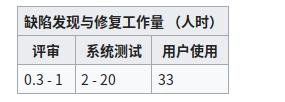
\includegraphics[width=10cm]{Screenshotfrom2022-01-1801.jpg}

但很多研发团队只依赖测试来保证质量,导致大部分缺陷都要等到系统测试甚至客户验收时才被发现。

\framebox{%
\begin{minipage}[t]{0.97\columnwidth}\raggedright
如何通过提高评审效率来降低质量成本 (Economics of Software Quality)
质量成本由三部分组成:

\begin{enumerate}
\tightlist
\item
  失效(Failure)成本\\
  把缺陷修复好的成本,包括在客户现场被发现的缺陷。
\item
  评测(Appraisal)成本\\
  包括各类测试,如系统测试,集成测试,单元测试等,所花的工时
\item
  预防(Prevention)成本\\
  包括技术评审 (注:有些人把评审归为评测成本,这里按 Mr.Juran
  定义,归属于预防成本)
\end{enumerate}

加大预防(评审)的力度,可大大减少失效成本(如测试和验收工作量)

例如,开发10万行代码(包含新增和变更):\\
场景1:评审效率只有50\%:\\
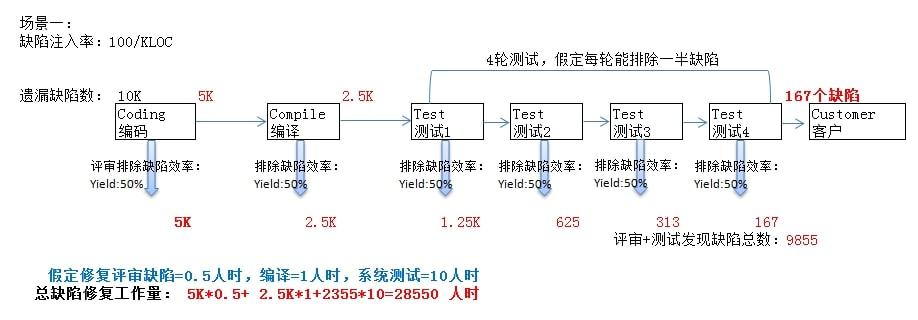
\includegraphics[width=8cm]{缺陷场景1_2_0.jpg}\\
场景2:评审效率达到75\%:\\
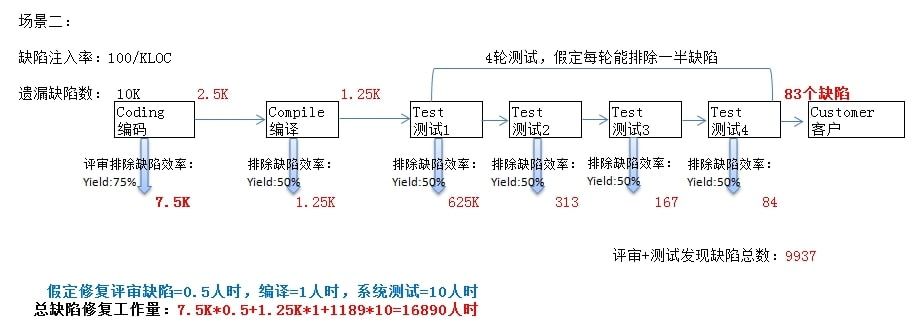
\includegraphics[width=8cm]{缺陷场景2_2_0.jpg}\\
\strut
\end{minipage}}

从以上例子看到,提高评审效率不仅能把交付给客户的缺陷减半 ,
更重要的是能够降低质量成本的失效成本,为了提高评审效率,工作量可能会略有增加,评测成本基本不变
。 把代码评审效率从50\% 提升到75\% 便能节省 1,462 人天 {[}=(
28.5-16.9)/8{]} (假定1人天=8小时),节省超过40\%。注意:场景1与2
过程中评审或测试排除数基本不变,同样大概 9.9K,只是场景2
把2.5K测试缺陷推前在评审发现,但因修复系统测试缺陷要10人时,但修复评审缺陷只需0.5人时。不同公司的缺陷修复工作量可能不同,但只要后面系统测试缺陷修复的工作量比评审的工作量大,那么把缺陷从后面的测试前移到评审发现,便能大大减少返工的工作量。

评审通常包括需求、设计、代码
评审,另外可以增加架构评审,原型评审。例如,如需求评审有客户参与,效率/效果都会更好。

总监开心地说:对了,我们开发好像一直都没有太注意评审,
觉得浪费时间,也没有评审出多少缺陷。
听你的例子,只是把评审效率从50\%提高到75\%便可以降低四成成本,如我们能从0\%升到50\%应该也能节省不少,我觉得降低一百万这目标应该有希望了。
我马上要求质量部发布评审规范与过程,并要求每一个团队都必须按这个去做。\\
问:这个例子中的质量成本(主要是失效成本)降低了四成,虽然未包括开发本身成本,但确实也省了不少。但请注意改变人的习惯很艰难,不能单靠发布流程。
必须先从个人习惯入手。你估计导致质量成本增加的主要原因是什么?

总监答:很多原因,例如前面需求没做好导致设计编码有误。

我说:去年一家我们辅导的公司,每次做完迭代冲刺后,都会叫上所有组员,包括产品经理、测试开发一起看看本次迭代的问题,讨论一下那几十个缺陷是源自哪方面?是否因为需求没做好?还是开发编码本身的问题?针对当次回顾复盘反馈最多的问题,并讨论它的根因后,在下一个迭代中采取一些针对性的改进措施,希望下一个迭代能减少对应的系统测试问题。\\
例如,有一次回顾时候就发现有一个功能升级模板,因为产品经理没有把握好客户的实际要求,导致我们那次迭代做出来这个功能不满足客户要求。虽然有做需求评审,但大家未能发现这需求问题。过程改进组就更新了需求评审检查单,增加一项,希望以后会减少同样的问题。另外,我们发现除了需求以外,还有很多是因为代码本身写得不规范,比如,有很多分支,常数也没有处理好。这些都在后面的系统测试和一些客户发现的问题反映出来。改进组便相应地加强了代码评审和代码规范的检查项和样例,来避免再发生同类问题。\\
总监问:有什么效果?\\
我答:其实大部分的缺陷都是人的缺陷防范意识弱,经过几轮培训与辅导,大家便更注意,主管也开始注重,后面的迭代,这类的问题就减少,不再是主要问题。\\
你们现在不是要求项目组在每个冲刺(迭代)后都必须要做个小组内部回顾吗?可否安排我参加,观察一下。\\
总监:正好我们下午应该有一个项目组要做内部回顾复盘(Retrospective),欢迎您来看看。

\hypertarget{ux4eceux9879ux76eeux51b2ux523aux7684ux56deux987eux590dux76d8ux5f00ux59cb}{%
\subsection{从项目冲刺的回顾复盘开始}\label{ux4eceux9879ux76eeux51b2ux523aux7684ux56deux987eux590dux76d8ux5f00ux59cb}}

在回顾复盘现场,测试人员投影了本次迭代的缺陷分析,展示下面两个缺陷分布图
:

\begin{itemize}
\tightlist
\item
  开发人员排名(最多的排头)
\item
  按模块来区分(最多的排头)
\end{itemize}

团队组长便按照缺陷的严重程度询问每位开发人员 -\/- 是否知道怎么修改?\\
大家都说知道了。组长要求大家提出问题,如果没有问题就准备散会。

我问:大家好,你们有没有兴趣做个``整个团队一起改善整个系统''实验。
后面让我们暂时抛开自己本身是什么岗位。
大家一起看看有哪些地方能减少缺陷?

例如,除了按照人员与模块区分。 我们可否把缺陷简单按下面类型分组 :
需求/设计/编码 ?

他们就让测试人员,展示本冲刺发现的34个缺陷,让大家逐一讨论,找出缺陷是源自哪过程
,最后把总数写在在白板上:


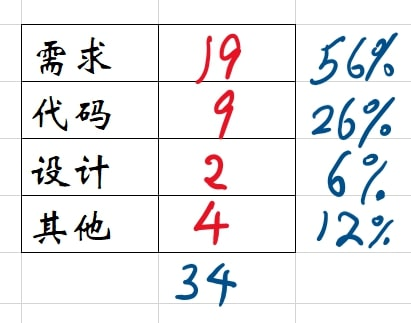
\includegraphics[width=10cm]{DefectsBySourceScreenshot_2021-09-20_155232.jpg}

让我们看看是怎么分布? 为什么这类缺陷最多呢?大家估计背后是什么原因?
针对需求(最多的类别),我辅导团队利用KJ方法{[}详见附件A2{]},识别主因。最终汇总成以下结果:\\

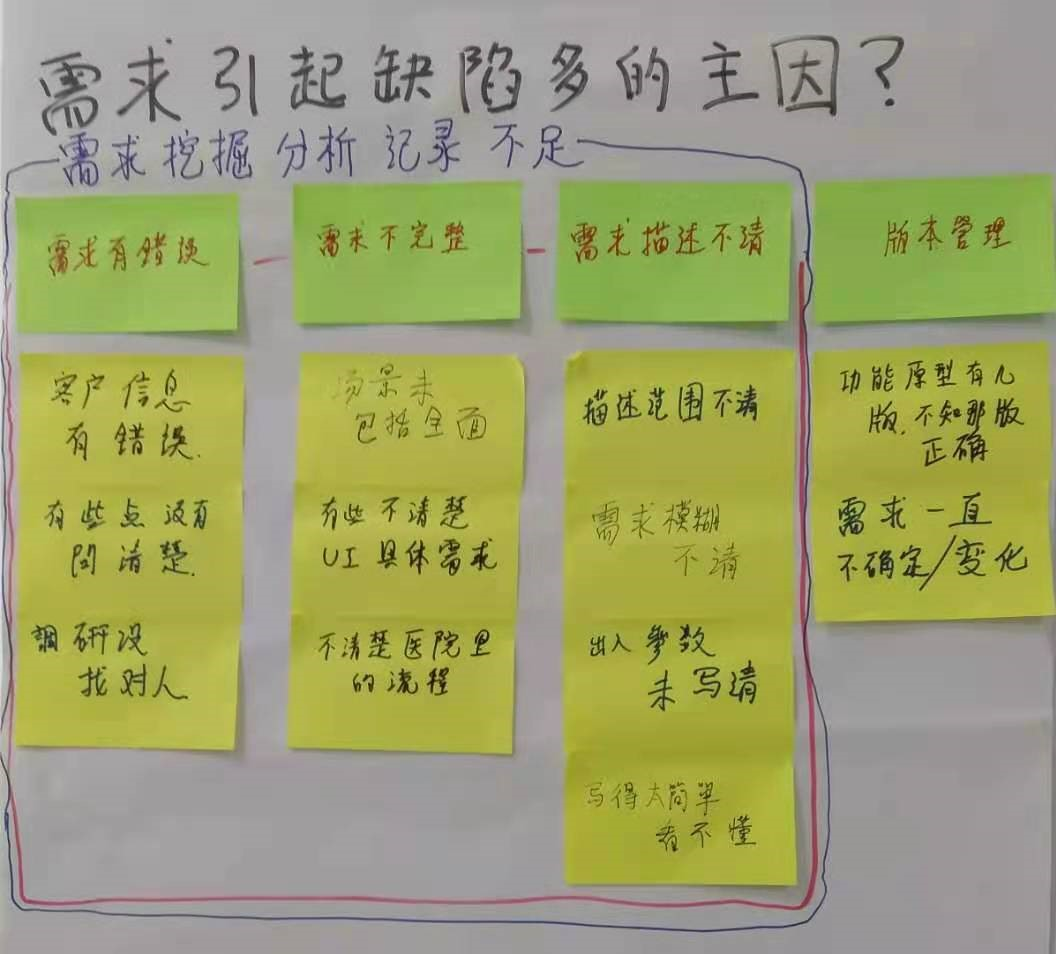
\includegraphics[width=10cm]{微信图片_20210920125228.jpg}

\hypertarget{ux4eceux95eeux9898ux5206ux6790ux5230ux6839ux672cux539fux56e0ux5230ux884cux52a8}{%
\subsubsection{从问题分析到根本原因到行动}\label{ux4eceux95eeux9898ux5206ux6790ux5230ux6839ux672cux539fux56e0ux5230ux884cux52a8}}

我问:针对我们刚才一起找出的主因,根本原因是什么?
如何可以避免同类缺陷再发生?

答:要加强对需求人员的培训,提高他们的能力。\\
总监说:我年初已察觉到确实很多需求没有表达清楚。
导致开发出来的东西不符合客户要求,或不是客户要的。

我见过以下用户故事:

\texttt{病人或他的家属能容易找到他选择的服务。}\\
\texttt{~理由:他们熟悉网上购物,习惯了方便和快速的响应时间时间。}~\\

我问需求人员怎样才算容易找到,验收标准?

我估计她记得我说过需求必须可测量,她想了一会,说:验收标准:``普通病人能够在6秒钟内通过不超过三个动作定位任意一项服务。''

我说如果把`普通病人'改为`90\%以上的病人'更好。

必须把模糊,有二义性的需求变成可以测量。

所以不能仅仅说 `新功能很酷,很创新',
而应明确验收标准为:引入了新功能的三个月之内,60\%的用户应该用它来完成规定的工作。75\%以上的用户对产品表示赞许。

所以三个月前,我已经开始 准备正式规划产品经理与需求分析师岗位:
要经过挑选,考试,然后培训,达标才能正式上岗。
本来计划两周后会正式公告,现在既然你们问到,我就预告一下。

我说:既然高层已经有长远的规划,我们团队就应该针对下一个
冲刺,我们可以做到的事情。

项目经理说:我们每个岗位都已经尽了全力,没有什么可以做了。\\
我问:你们有做评审吗?如需求,设计评审\\
答:有。\\
问:需求评审发现多少缺陷,设计评审发现多少?\\
答:好像两三个。\\
问:发现什么问题?\\
答:记不清了,当时直接就修改了。\\
问:请问评审总共花了多少时间?多少人参加?\\
答:我们六个人,那次评审大概用了接近2小时。\\
问:2小时?\\
答:我们不仅仅发现需求问题,也一起讨论如何修改\\
问:如果评审只找缺陷,记录,应不会超过一小时,如果大家事前做好准备,估计可能半小时可以完成。所以通常检查(Inspection
)不会当场讨论如何修改。\\
我接着说:我们刚才分析系统测试缺陷,不是识别出超过一半是源自需求吗?为什么我们不能在评审时预先发现?
你们觉得可以下一个冲刺,评审时可以发现更多缺陷吗?\\

\texttt{我立马用5分钟与大家分享有效评审能降提高产品质量,降低成本的例子。}

答:估计应该可以,但不知道怎么做?\\
问:你们评审有检查清单吗?\\
答:没有。\\
问:清单可以帮助我们吸收以往的经验,避免以后同类问题再发生。
例如刚才我们都识别了跟需求挖掘/分析/记录不足相关的具体问题吗?
可否利用这些,更新评审检查单的检查项项,提醒我们要避免同类问题。
如果大家同意,我们现在就行动。我们要改进
便要制定目标,例如计划下次需求评审,系统测试等各过程发现的缺陷数。
这些目标你们可以下周一策划两周冲刺时定。

\texttt{组长安排了小李更新检查单。准备在下次评审前与需求文档,预先发给参评人员。}

我说:谢谢大家,我没有其他要说了,下次回顾,我或总监会来参加,看看冲刺的效果。

\framebox{%
\begin{minipage}[t]{0.97\columnwidth}\raggedright
冲刺回顾与根因分析 回顾时对本冲刺的数据做根本原因分析
是持续改进的最佳实践。\\
我在这案例是按下图的五步来辅导团队,确保
每一位成员都全心投入参与,并从分析形成行动,达到改进效果:\\
\#设置舞台

\begin{enumerate}
\tightlist
\item
  收集数据
\item
  分析,找出根因
\item
  决定做什么
\item
  结束
\end{enumerate}

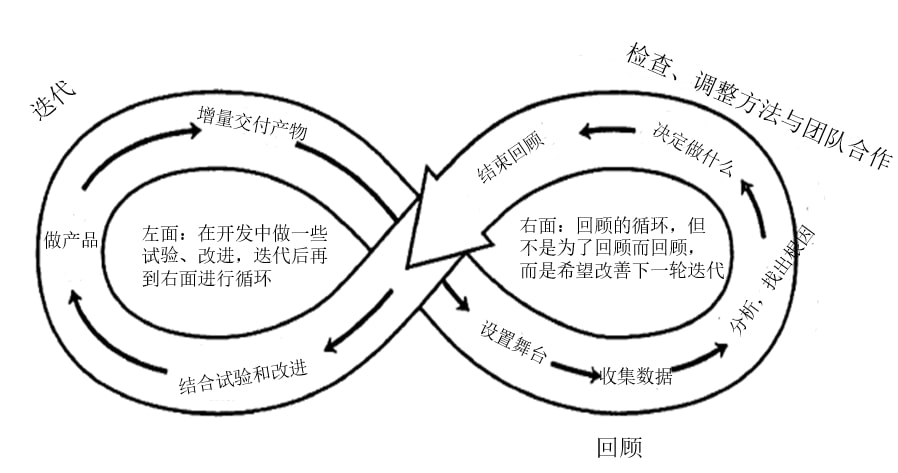
\includegraphics[width=10cm]{RetrospectiveScreenshot_2021-09-21_173119.jpg}\strut
\end{minipage}}

\hypertarget{ux6539ux8fdbux8981ux4eceux4e2aux4ebaux6570ux636eux7edfux8ba1ux5165ux624b}{%
\subsubsection{改进要从个人数据统计入手}\label{ux6539ux8fdbux8981ux4eceux4e2aux4ebaux6570ux636eux7edfux8ba1ux5165ux624b}}

复盘会后,我找了团队的两位开发,她们都是在开发岗位工作了4、5年的女编程员,一位叫小萍(XP)
, 另一位叫`Shirley'(S)

我问:大家觉得刚才回顾会后面的讨论怎么样?\\
XP过了一会说:以前回顾会都是问责,我们做开发的都不敢发言,说多错多。
因为是我负责的模块缺陷偏多,我肯定不愿意在大家面前丢脸。 到后面用
写便利贴方法
(她是指KJ法),我就不怕直说了,其实以往的回顾会都是主持人(项目经理)
讲,我们只是听。

我问:你们觉得刚才在回顾里提到可利用加强评审来减少后面缺陷的返工怎样?\\
XP:
有道理,但现在测试工具都很先进,立马就可以把缺陷暴露出来,为什么还需要
依靠人工查看代码,这样做不是更耗费时间吗?\\
问:好的,首先让我先理解你们现在的开发过程?\\
答:写代码编辑,先自己编译通过,然后自己手工测试一下。\\
(她们的表情好像在说:还听其他组员说您是软件工程20年经验的专家,还会问我这些低级问题?)\\
问:测试之前有没有做设计或代码的评审。\\
答:没有,因为时间都很紧,手工评审很耗时。\\
问:理解。但软件工程界统计过如果同样的缺陷等到系统测试才被发现,可能要好几天才能解决,但如果能在代码评审(或需求评审)中被发现,很可能不到30分钟便能解决。\\
一般情况下,你们需要花多少时间修复在系统测试阶段发现的缺陷?\\
答:没有正式统计过,差不多半天到好几天都有。\\
问:如果像Apache,Eclipse
那类超大型软件,很可能不止。如果要找出答案,便需要数据。
例如,我们现在关心:缺陷数,评审工作量,缺陷修复工作量。
必须要求每人在开发时,自己把数据记录下来,
以数据说话,到后面才知道有没有提升,返工工作量有没有减小。
虽然通过评审尽可能早地发现缺陷是最好的,
但不能只依赖评审,必须也有单元测试。 与评审一样,
单元测试也能帮助我们提前找出缺陷。

S:现在我们都已经用敏捷开发了, 同行评审好像都是上一代瀑布开发年代的事情,
是否已经过时?\\
我说:虽然敏捷好像不强调评审,但极限编程 (eXtreme Programming)
里有结对编程 (Pair Programming) ,
其实也是一种评审。只不过不是等到写完代码后才评审,
编码的同时有人在评审, 所以敏捷并非没有评审,
目的都是希望尽早发现缺陷,防止遗漏到系统测试阶段。
如果你们能在编码时能减少缺陷, 也同样能达到减少缺陷遗漏的目的.\\
S:是否应该通过测试后才评审代码?便可以针对有问题的代码,节省工作量?\\
我说:这个思路看来好像不错,但最大的问题是这会影响评审组找出缺陷的动力。因评审员都知道这软件已经测试过。\\
S:好吧,再前一步,是否应该在通过编译后才评审代码?\\
A:虽然各有长短。我建议先评审,后编译\\
例如编译通过不表示所有的编码格式问题都被找到。
你们都不会再去关注代码的格式问题了,从而导致那些问题(可能10\%)要到系统测试阶段才暴露出来。\\
我问:你们哪位知道如何制定锻炼计划准备六个月后可以参加半马比赛?\\
(S高高瘦瘦很运动型,我猜可能她知道。)\\
XP:必须制定很详细的每周锻炼流程,度量每次的时间、速度。\\
(后来我才知道XP她刚跑完半马,人不可以貌相)

我问:要提升个人的编码能力(质量,效率)就与准备马拉松一样,天天收集数据才知道新方法是否有帮助,有没有改善。你们有兴趣吗?\\
XP答:OK ,但S和我写不同的模块,收集数据是否只是供自己作前后比较?\\
我说:
很好的问题。两个月前,我们陈老师不是教你们用简化功能点来衡量项目规模吗?
如果像你们每个项目都使用功能点,你们的缺陷密度就有可比性了。

XP:如何收集汇总缺陷,统计数据?\\
我说:先由开发人员自己记录,然后在回顾时,由项目经理和组长统一汇总到公司项目数据库中。
大家也可以利用回顾,看看现在和以往的数据趋势,一起分析讨论。\\
我接着说:你们可以按照以下这个数据模板,记录下通过测试与评审发现的缺陷数量,与返工工作量,然后我们做统计分析。
看看评审能不能帮到你们降低修复缺陷的工作量,最终能提高你的代码生产率。以下是以前两位编码人员的个人统计,可以看到如果能通过代码评审发现缺陷,代码生产率就越高:

\includegraphics[width=6cm]{hump291Fig913Student1_2_0.jpg}\\
\includegraphics[width=6cm]{hump292Fig914student2_2_0.jpg}

Key: 评审效率 Yield = 代码评审找出缺陷数 / 代码引起缺陷总数
(=评审找出缺陷数+后期测试发现的缺陷数)\\
:: 生产率 = 每人每周产出多少有效功能点 (FP)\\
你们后面也可以自己做出类似的图。\\
XP:听起来收集数据要花不少工作量,有软件工具自动收集吗?\\
我问:请问你跑半马前,如何做准备?\\
XP:比赛前六个月开始按定好的计划训练,并记录每次实际时间。\\
问:怎样记录?\\
XP:现代跑步的都有电子数字手表,记录每段的开始与结束时间,很简单。\\
我说:统计个人实际工时也类似,编码时记录开始与结束时间,不需要自动化工具。你也可以看看我以前的经验分享《个人如何写程序并记录》\\
难点不是在收集数据花多少时间,而是改变个人的习惯,您刚开始锻炼时估计也应遇过同类问题?\\
XP:是的,好在我们有个跑步团,我看大家都这样做,我慢慢便习惯了。\\
我接着总结说:当你们收集了多轮数据后,便可以分析并制定提升代码质量的策略:\\
每人都有各自的长短。 有了自己的缺陷统计数据后。 改进必须有针对性:
哪一类的缺陷出现最多最严重? 应选择哪个最弱的过程才容易有效果。

最后,预防胜于治疗,最终不能单靠评审与测试,更需要在编码时,注意避免引入缺陷。
真是没有必赢的金科玉律,但有数据才有动力,才有方向,促进改变以往的习惯。
好比减肥,必须每天测量自己的体重一样。
(我看她们的两位体重都正常,应该可以提这个对女性较敏感的题目。)

\hypertarget{ux5efaux7acbux516cux53f8ux5ea6ux91cfux6807ux6746ux57faux7ebfux4e0eux6a21ux578b}{%
\section{建立公司度量标杆(基线)与模型}\label{ux5efaux7acbux516cux53f8ux5ea6ux91cfux6807ux6746ux57faux7ebfux4e0eux6a21ux578b}}

四个月后,每项目组收集了五六轮数据。公司过程改进组长问如何分析数据建立公司基线。

我们就看了两个项目的迭代缺陷密度趋势图:

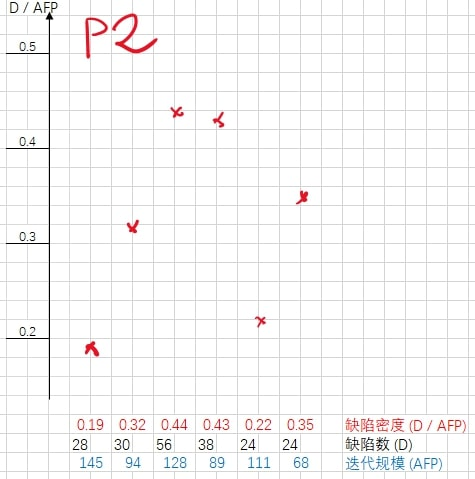
\includegraphics[width=6cm]{P2CcScreenshot_2021-09-25_111304.jpg}
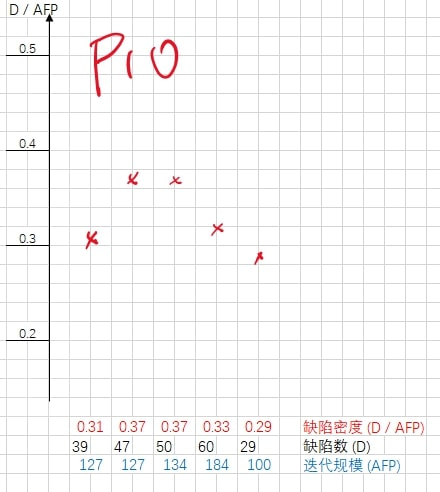
\includegraphics[width=6cm]{P10CcScreenshot_2021-09-25_104057.jpg}

我问:你觉得怎么样?是否稳定?可否建立基线?(希望他可以自己找出答案,不仅仅听我的。)

他说:觉得P10比较好,波动的幅度不大,P2的差异太大了。\\
我说:是的,波动这么大,其实不用画控制图。\\
应先问问P2 项目经理变化这么大(68 -
145)的原因。确保数据正确之后,才可以分析数据,建立基线。其实这些项目数据量都不够。
虽然如此,你还是可以告知两项目组这初步分析结果,但必须要提醒他们数据还未稳定下来。
还记得我们培训时讲过以下基线例子,当过程已经稳定后(没有异常点),
如有异常波动超越了控制图上下线范围,表示过程可能有基本变化。
当变化后的过程稳定下来后,我们便需要更新基线。


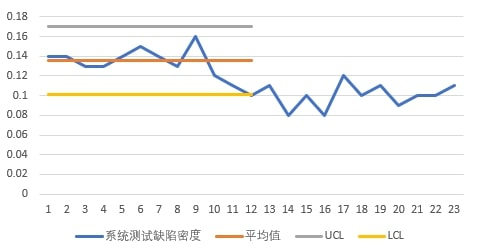
\includegraphics[width=6cm]{925BeforeScreenshot_2021-09-25_115004.jpg}
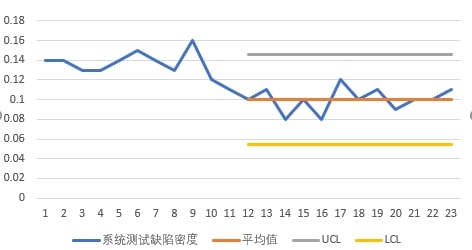
\includegraphics[width=6cm]{925AfterScreenshot_2021-09-25_115237.jpg}

{[}详见附件A3: 如何画ImR控制图{]}

\hypertarget{ux5206ux6790ux9879ux76eeux6570ux636eux5efaux57faux7ebf}{%
\subsection{分析项目数据,建基线}\label{ux5206ux6790ux9879ux76eeux6570ux636eux5efaux57faux7ebf}}

我问过程改进组长: 你们如何得出基线的?有什么分析?\\
答:这个就是我们各项目每个迭代的数据收集表,我就把以往所有项目的每迭代数据,统计所有数据,得出Q1(P25)、Q2(P50)跟Q3(P75)的数,成为我们的基线。\\
问:你有没有分析这些数据?会不会不同的项目之间不一样,导致你的总的基线需要细分一下呢?\\
然后我就举了一个我们用来培训的例子,对70个项目,收集了各种缺陷的统计,我们总体把缺陷归纳成7种类型。如我们按那个7种类型,各自看他的象限图的时候,明显看到他们是之间是有区分的,不能合并成一个基线,如果合并成一个基线,那整个基线的范围就太宽了,没有什么好的参考作用。从最低的0.3左右到最高的0.7。但是如果我们分成7组基线的话,每个基线的范围就窄很多,更有参考作用。\\

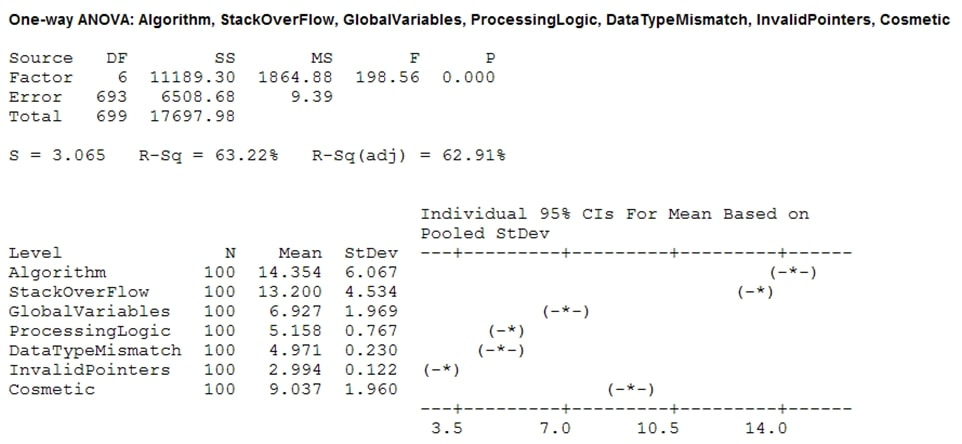
\includegraphics[width=10cm]{Opp_3.jpg}

所以我们就简单地依据公司的不同项目,画出各项目的缺陷密度,看看是怎么分布。\\
问:所以你的基线不应该只是看所有的范围,而应该是针对这个稳定的取一个基线,针对这个这两个项目去考虑比较。因为这种比较稳定的项目数据基线,才更有参考作用。加入其它的项目只可能加宽基线范围,对后面项目作参考没有好处。\\
我再问:有了基线以后,你如何依据商业目标去制定你下个月的质量目标?\\
答:从商业目标,我们可以推算出缺陷数或者缺陷密度大概是什么水平?我们统计一下,平均一个缺陷的修复成本是112元左右。所以这个商业目标就可以帮我们知道,从业务目标每个月的缺陷密度要多少才可以有可能最终达到整年的成本降低计划。\\
我说:好啊,有了这个从业务目标得出的质量目标后,你怎么制定改进行动以达到规定成本降低目标?因为如果你没有什么基本的改变,理论上,缺陷密度或者缺陷数是不会降的。\\
我问:你们除了收集数据,有没有把过去每个迭代的质量相关数据标注在生产力发展趋势图上,让你们个人与团队都可以看到过去的变化?如果团队里个人之间的差异很大,这情况可能会按每个人统计更准确。

\hypertarget{ux57faux7ebfux6570ux636eux5206ux6790}{%
\subsection{基线数据分析}\label{ux57faux7ebfux6570ux636eux5206ux6790}}

我说:分析后,可以比较不同项目之间基线范围的差异。
判断项目之间的差异有多大?是否合适归纳成一个总的公司基线。

除了按项目细分,也可以按其他维度细分(例如,按各种缺陷类型的比例。)帮你回答以下问题:

\begin{itemize}
\tightlist
\item
  系统测试 / 验收测试缺陷从前面那个阶段遗漏下来
\item
  代码评审的效率(Yield)
\item
  效率是否跟缺陷种类相关?
\end{itemize}

如果差异很显著,就不需要使用 方差分析(超过2组) , 双样本 T检验
(2组)方法判断分组有没有显著区分。

\hypertarget{ux5229ux7528ux57faux7ebfux4e0eux6a21ux578bux5236ux5b9aux8d28ux91cfux8ba1ux5212}{%
\section{利用基线与模型制定质量计划}\label{ux5229ux7528ux57faux7ebfux4e0eux6a21ux578bux5236ux5b9aux8d28ux91cfux8ba1ux5212}}

要降低最终测试缺陷率,不能单靠不断提醒自己要努力。
要提升,也可以利用80:20原则, 针对占比最多的缺陷类型入手。

我们发现不良分支类占比最多。
过程改进组使用KJ头脑风暴法,找出根本原因,并用加强评测/预防来减少失效质量成本的思路,得出以下对应纠正措施:

\begin{itemize}
\tightlist
\item
  评测

  \begin{itemize}
  \tightlist
  \item
    完善评审检查单,增加与不良分支相关的检查项希望能在评审时检测出来。
  \end{itemize}
\end{itemize}

\begin{itemize}
\tightlist
\item
  预防
\end{itemize}

\begin{description}
\tightlist
\item[]
对应以下四大类根因种类的改进措施:
\end{description}

\begin{enumerate}
\tightlist
\item
  教育/培训 education 编码规范与培训没有明确要求
\item
  个人疏忽 oversight 忽略了要尽量避免不良分支
\item
  执行 transcript 因不良分支不是语法错误,IDE与静态检查代码都没有发现
\item
  团队沟通 Communication 组长安排编程任务与查看代码时没有注意
\end{enumerate}

大家讨论后,除了改善规范检查单与培训外,也决定写个代码扫描小程序来暴露和数代码里这类问题,不仅仅靠人工评审查看。

\begin{description}
\tightlist
\item[]
= = = =
\end{description}

基于从项目收集的数据 - 每一个阶段的缺陷数,返工工作量范围,
过程改进组建立了一个水晶球蒙地卡罗预测模型{[}详见附件A5{]}:
例如对每一个迭代

\begin{itemize}
\tightlist
\item
  输入本迭代动态功能点数(规模)与各过程(需求/设计/编码)的缺陷率(引入多少缺陷)
\item
  输入需求评审各种方法的评审工作量和预估评审效率
\item
  输入设计评审各种方法的评审工作量和预估评审效率
\item
  输入代码评审各种方法的评审工作量和预估评审效率
\item
  输入代码单元测试的缺陷排除率
\item
  输入系统测试的缺陷排除率
\item
  模型便预测系统测试后的遗漏缺陷数,与返工工作量
\end{itemize}

因为要提高评审效率需要花工作量,
这模型就可以帮我们比较:哪个过程,使用什么评审方法,目标的评审效率,对缺陷数和质量成本的效果。

开始的时候,项目经理只能依赖经验来估算,现在有了公司的基线预测模型与性能目标要求作参考,便可以更好地制定本迭代的质量目标(各个过程,包括系统测试要发现多少缺陷
和相关的评审方法)。

无论是基线,或模型都是有它们的局限和不确定性。
所以项目经理会除了参考极限与模型的预测外,还是会依据经验,综合考虑来制定量化目标和选用那种方法。


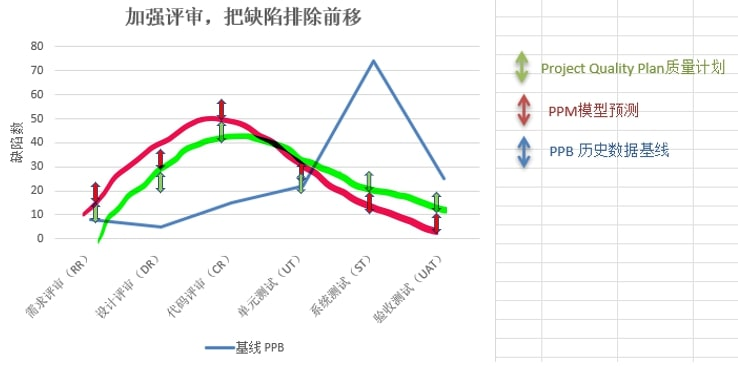
\includegraphics[width=10cm]{MoveDefectsForwardScreenshot_2021-11-18_215056.jpg}

Key: 蓝色是以往的基线 - 绝大部分缺陷都是在系统测试才发现;
浅绿色是量化质量计划的缺陷率目标 -
参考PPM(红线),计划利用提高前期评审的效率,减少系统测试与验收缺陷密度\\

\framebox{%
\begin{minipage}[t]{0.97\columnwidth}\raggedright
制定质量计划 (Quality Plan)

\begin{itemize}
\tightlist
\item
  从需求到设计、编码,如果方法没有变化,项目质量也不会改变。以代码评审为例,质量计划也要明确什么过程,选择哪一种评审方式。例如一般前端的代码,并非核心,使用简单的一对一或者代码扫描便可以了;但对于一些有逻辑处理的核心模块,可能需要用正式会议评审才能有效地找出大部分缺陷。
\item
  现在回顾复盘不像以前只是讨论哪些缺陷?哪些模块有问题?交给哪个开发去跟踪并处理?
\item
  开发成员看到团队的趋势数据,就会想不断提升,保持和以往一样的同一个水平也不行,现在团队包括每一个成员都会关注质量生产率指标。
\end{itemize}\strut
\end{minipage}}

\hypertarget{ux66f4ux65b0ux91cfux5316ux6027ux80fdux76eeux6807}{%
\section{更新量化性能目标}\label{ux66f4ux65b0ux91cfux5316ux6027ux80fdux76eeux6807}}

我问过程改进组长:还记得六个月前,我问你们的改进目标吗?\\
答:当然记得,要降低开发成本一百万\\
我们刚做了回顾,从项目数据,基线,预测模型,并更新了目标。下图从高层目标关连到研发性能目标QPPO
:\\


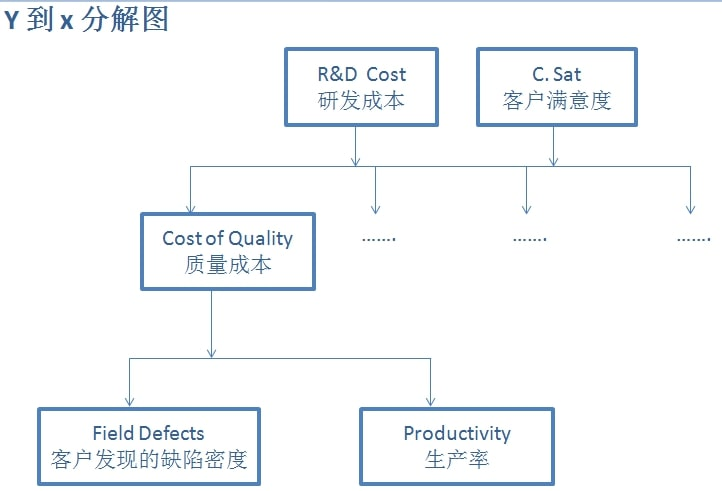
\includegraphics[width=10cm]{目标上下关系图.jpg}

我问:挺好,你们如何把高层的业务目标关联到开发团队的性能目标QPPO?\\
答:以前没有太多数据,到了3月份,我们就依据过去6个月的数据得出缺陷密度的基线------Q1:
0.27、Q2: 0.35、Q3: 0.41 (Note1)。依据这个基线,制定4月份的QPPO目标是Q1:
0.25,Q2: 0.34、Q3:
0.47,因为我们觉得中位数应该有些下降,但是不是每一个项目都具备强配合能力,所以估计向下那个范围还是跟以前差不多。\\
::Note1: Q2=中位数 50 percentile,或叫P50 ; Q1= 25 percentile,P25 ; Q3=
75 percentile,P75

制定性能目标除了要有分布范围,例如 Q1 / Q2 / Q3 , 不再是以前升10\%
的那种单点目标:\\
以前单点的话只会说均值从X\%降到Y\%(eg.来年希望降低质量成本25\%)。但不会像这种从Q1、Q2、Q3,不仅考虑中位数也考虑范围。以前单点时可以说,是否达到预期的目标,只看中位数。这种考虑不够全面。现在我们有分布的概念,当被问到预期目标完成情况时,我们会说Q1达不到,跟以前一样,Q3也没有什么变化,但我们Q2
是达到本来预期目标。\\

\hypertarget{ux6539ux8fdbux6548ux679c}{%
\section{改进效果}\label{ux6539ux8fdbux6548ux679c}}

从建立第一轮基线后,过了三个月,过程改进组分析8个试点项目的改进效果,准备汇报给高层,发现8个项目的数据差异还是很大。其中有2个项目很明显看到有质量的提升、系统测试缺陷的降低、返工量的降低。有三个项目数据不全,而且也没看到太大的变化。有两个项目几乎就没有提供数据,过程改进组分析原因,发现和这个项目组的领导有关,两个有效果的项目,他的领导一直积极支持量化管理过程改进。\\
我看过程改进组好像对结果有点失望,就跟大家打打气说:\\
大家千万不要以为过程改进的路很简单,开始的时候反对声音大是很正常的,因为要改变一个人的习惯是很难的,但起码从这几个月的实验数据来看,我们的量化管理是有效果的。后面我们就可以利用这两个项目的经验,开始后面的改进。管理层监督都应该以数据说话,不应该只是听高层管理的一言堂。我相信再过几个月,会有越来越多项目组采用这个方式来加强管理。丰田的大野赖一先生在50年代推动精益管理时,也不是所有的主管听他这一套,但他一直坚持下来。现在不仅丰田,其他的日本汽车公司都以丰田生产方式(Just
in time) 生产汽车,成为世界级的汽车生产流程。\\

\hypertarget{ux603bux7ed3}{%
\subsection{总结}\label{ux603bux7ed3}}

\begin{enumerate}
\tightlist
\item
  单靠统计分析是不会提高开发质量的,必须找到对应的方式,例如注重同行评审,不要等到系统测试才发现缺陷。
\item
  做好需求以减少设计与编码对需求的误解。
\item
  统计数据让开发人员可以``看到''到现在的状态与趋势,且分析新方法对提升有没有作用。
\end{enumerate}

\textbf{这案例主要方法与重点}\\
1.目标要满足SMART\^{} 原则,目标有分布的概念\\
::\^{}(S=具体 M=可度量 A=可实现 R=相关的 T=有时间 )
2.降低质量成本的方法:\\
定期复盘造成本次缺陷最多的原因,是需求原因还是编码过程不规范:从而加强代码评审和规范性检查,还是完善需求评审检查单。

3.质量抓重点:例如一般前端的代码。并非核心,使用简单的一对一评审或者代码扫描便可以了;但对于一些有逻辑处理的核心模块,可能需要用正式会议评审才能有效地找出大部分缺陷

4.检查单可弥补经验的不均衡。

5.收集个人数据\\
主要依赖手工收集,因很多是无法靠系统自动识别的 ,如缺陷源自哪个过程。

6.利用水晶球预测模型,帮项目组在策划时找最佳配搭


\cite{MA2References1}

